\documentclass[11pt]{article}
\usepackage[margin=1in]{geometry}
\usepackage{graphicx}
\usepackage{booktabs}
\usepackage{array}
\usepackage{hyperref}
\usepackage{caption}
\usepackage{float}
\raggedbottom
\emergencystretch=2em
\renewcommand{\tablename}{Supplementary Table}
\renewcommand{\figurename}{Supplementary Figure}
\renewcommand{\thetable}{S\arabic{table}}
\renewcommand{\thefigure}{S\arabic{figure}}
\renewcommand{\theHtable}{S\arabic{table}}
\renewcommand{\theHfigure}{S\arabic{figure}}

\begin{document}

\begin{center}
{\Large\bfseries Supplementary information}\\[0.75em]
{\large Reproductive life-course phenotyping in the National Survey of Family Growth: a self-supervised temporal survey study}\\[0.75em]
Feifan Lu, Fengshang Yan, Qianqian Yang, Jiuqiong Yan, Rui Guan
\end{center}

\section*{Supplementary tables}

Supplementary Table S1 through Supplementary Table S11 provide numerical source summaries for cluster selection, endpoint enrichment intervals, age-range sensitivity, covariate adjustment, baseline methods, leakage sensitivity, subgroup robustness, the ever-pregnant stratum, simple age/parity baselines, raw-feature versus SSL supervised comparisons, and encoder seed sensitivity.

\begin{table}[H]
\centering
\caption{Development-cycle cluster selection metrics across k=2--8.}
\label{tab:cluster_selection}
\scriptsize
\setlength{\tabcolsep}{3pt}
\begin{tabular*}{\textwidth}{@{\extracolsep{\fill}}rrrrrrr@{}}
\toprule
k & Silhouette & DBI & Min. cluster, \% & Boot. ARI & Boot. n & Selected \\
\midrule
2 & 0.587 & 0.617 & 43.3 & 0.999 & 60 & False \\
3 & 0.606 & 0.701 & 4.6 & 0.914 & 60 & True \\
4 & 0.518 & 0.720 & 4.7 & 0.738 & 60 & False \\
5 & 0.385 & 0.969 & 4.0 & 0.797 & 60 & False \\
6 & 0.385 & 0.953 & 1.6 & 0.780 & 60 & False \\
7 & 0.366 & 1.040 & 3.2 & 0.750 & 60 & False \\
8 & 0.366 & 1.029 & 1.5 & 0.715 & 60 & False \\
\bottomrule
\end{tabular*}
\end{table}


\begin{table}[H]
\centering
\caption{Full temporal-validation phenotype-by-endpoint enrichment with bootstrap intervals. Intervals are stratified cluster percentile bootstrap intervals using public-use \texttt{VEST}/\texttt{VECL} design variables with respondent weights retained.}
\label{tab:endpoint_enrichment_ci}
\scriptsize
\setlength{\tabcolsep}{2pt}
\begin{tabular*}{\textwidth}{@{\extracolsep{\fill}}>{\raggedright\arraybackslash}p{0.19\textwidth}crr>{\raggedright\arraybackslash}p{0.20\textwidth}>{\raggedright\arraybackslash}p{0.21\textwidth}@{}}
\toprule
Endpoint & Phenotype & Events & Prev., \% & PR (95\% CI) & RD, \% (95\% CI) \\
\midrule
Adverse proxy & P0 & 7 & 0.5 & 0.09 (0.01--0.19) & -4.9 (-5.7 to -4.1) \\
Adverse proxy & P1 & 219 & 9.2 & 1.72 (1.58--1.85) & 3.8 (3.0 to 4.7) \\
Adverse proxy & P2 & 48 & 22.2 & 4.13 (2.98--5.46) & 16.8 (10.7 to 24.0) \\
Contraceptive vuln. & P0 & 146 & 5.6 & 0.72 (0.63--0.81) & -2.2 (-2.9 to -1.5) \\
Contraceptive vuln. & P1 & 238 & 10.4 & 1.33 (1.22--1.44) & 2.6 (1.7 to 3.5) \\
Contraceptive vuln. & P2 & 21 & 7.6 & 0.97 (0.59--1.39) & -0.2 (-3.2 to 3.0) \\
Fertility/loss help & P0 & 114 & 4.3 & 0.39 (0.33--0.45) & -6.8 (-7.7 to -5.9) \\
Fertility/loss help & P1 & 397 & 18.2 & 1.64 (1.55--1.75) & 7.1 (6.1 to 8.4) \\
Fertility/loss help & P2 & 44 & 18.6 & 1.67 (1.19--2.19) & 7.5 (2.1 to 13.3) \\
Fecundity limit./infert. & P0 & 466 & 17.8 & 0.63 (0.58--0.68) & -10.3 (-11.9 to -8.7) \\
Fecundity limit./infert. & P1 & 807 & 38.8 & 1.38 (1.32--1.44) & 10.6 (9.0 to 12.3) \\
Fecundity limit./infert. & P2 & 94 & 41.0 & 1.46 (1.22--1.69) & 12.9 (6.2 to 19.3) \\
Mistimed/unwtd. & P0 & 51 & 2.3 & 0.07 (0.05--0.09) & -31.9 (-34.1 to -29.6) \\
Mistimed/unwtd. & P1 & 1,506 & 67.0 & 1.96 (1.88--2.05) & 32.8 (31.2 to 34.4) \\
Mistimed/unwtd. & P2 & 181 & 76.4 & 2.23 (2.06--2.43) & 42.2 (36.8 to 47.6) \\
\bottomrule
\end{tabular*}
\end{table}


\begin{table}[H]
\centering
\caption{Age-range sensitivity analysis in the 2022--2023 temporal-validation cycle. The phenotype with the highest 15--44 prevalence ratio for each endpoint is shown, then re-evaluated after including females aged 45--49 years. Phenotype assignment used the primary endpoint-excluded encoder without refitting; full-age assignment labels were aligned to the primary P0/P1/P2 labels by majority overlap in the original 15--44 subset, and reassignment agreement was checked only as a technical reproducibility control.}
\label{tab:age_sensitivity}
\scriptsize
\setlength{\tabcolsep}{2pt}
\begin{tabular*}{\textwidth}{@{\extracolsep{\fill}}>{\raggedright\arraybackslash}p{0.25\textwidth}crrrr>{\raggedright\arraybackslash}p{0.14\textwidth}@{}}
\toprule
Endpoint & Phenotype & 15--44 N & 15--44 PR & 15--49 N & 15--49 PR & Direction \\
\midrule
Contraceptive vulnerability & P1 & 2,228 & 1.33 & 2,691 & 1.26 & Same direction \\
Fertility or loss help & P2 & 239 & 1.68 & 315 & 1.35 & Same direction \\
Mistimed/unwanted pregnancy history & P2 & 239 & 2.23 & 315 & 1.98 & Same direction \\
Adverse pregnancy-history proxy & P2 & 239 & 4.11 & 315 & 3.25 & Same direction \\
Fecundity limitation/infertility & P2 & 239 & 1.47 & 315 & 1.34 & Same direction \\
\bottomrule
\end{tabular*}
\end{table}


\begin{table}[H]
\centering
\caption{Covariate-adjusted phenotype endpoint enrichment in 2022--2023. Models are survey-weighted one-vs-rest logistic enrichment models adjusted for age, race/ethnicity, education, poverty, insurance, and parity. Confidence intervals are stratified cluster percentile bootstrap intervals using public-use \texttt{VEST}/\texttt{VECL}. These models are descriptive robustness checks and are not causal models.}
\label{tab:adjusted_enrichment}
\scriptsize
\setlength{\tabcolsep}{3pt}
\begin{tabular*}{\textwidth}{@{\extracolsep{\fill}}>{\raggedright\arraybackslash}p{0.36\textwidth}crrc@{}}
\toprule
Endpoint & Phenotype & Adjusted OR & 95\% CI & Bootstrap n \\
\midrule
Adverse pregnancy-history proxy & P0 & 0.11 & 0.01--0.29 & 300 \\
Adverse pregnancy-history proxy & P1 & 1.65 & 1.04--2.85 & 300 \\
Adverse pregnancy-history proxy & P2 & 2.05 & 1.20--3.57 & 300 \\
Contraceptive vulnerability & P0 & 0.52 & 0.38--0.70 & 300 \\
Contraceptive vulnerability & P1 & 1.84 & 1.39--2.41 & 300 \\
Contraceptive vulnerability & P2 & 0.69 & 0.40--1.03 & 300 \\
Fertility or loss help & P0 & 0.25 & 0.17--0.33 & 300 \\
Fertility or loss help & P1 & 2.50 & 1.92--3.56 & 300 \\
Fertility or loss help & P2 & 1.23 & 0.78--1.86 & 300 \\
Fecundity limitation/infertility & P0 & 0.74 & 0.60--0.89 & 300 \\
Fecundity limitation/infertility & P1 & 1.25 & 1.05--1.52 & 300 \\
Fecundity limitation/infertility & P2 & 0.99 & 0.67--1.33 & 300 \\
Mistimed/unwanted pregnancy history & P0 & 0.02 & 0.01--0.03 & 300 \\
Mistimed/unwanted pregnancy history & P1 & 9.58 & 7.69--12.81 & 300 \\
Mistimed/unwanted pregnancy history & P2 & 2.25 & 1.56--3.47 & 300 \\
\bottomrule
\end{tabular*}
\end{table}


\begin{table}[H]
\centering
\caption{Baseline phenotyping method comparison in the 2022--2023 temporal-validation cycle. Mean maximum prevalence ratio is averaged across prespecified endpoints. Minimum cluster proportion and bootstrap ARI are development/test stability summaries; a high prevalence ratio from a very small cluster should not be interpreted as a stronger method.}
\label{tab:baseline_methods}
\scriptsize
\setlength{\tabcolsep}{3pt}
\begin{tabular*}{\textwidth}{@{\extracolsep{\fill}}>{\raggedright\arraybackslash}p{0.32\textwidth}rrrr@{}}
\toprule
Method & Mean max PR & Boot. ARI & Min. cluster, \% & Endpoints \\
\midrule
MCA-style one-hot SVD + k-means & 1.57 & 0.774 & 27.5 & 5 \\
Raw matrix PCA + k-means & 2.25 & 0.735 & 0.1 & 5 \\
SSL embedding + k-means & 2.16 & 0.953 & 4.9 & 5 \\
Selected-variable Bernoulli LCA & 1.50 & 0.904 & 18.5 & 5 \\
\bottomrule
\end{tabular*}
\end{table}


\begin{table}[H]
\centering
\caption{Endpoint-excluded versus full-domain encoder sensitivity. Values show the maximum phenotype prevalence ratio for each endpoint in 2022--2023. The primary endpoint-excluded encoder retained endpoint-enrichment patterns despite direct endpoint-variable exclusion.}
\label{tab:leakage_sensitivity}
\scriptsize
\setlength{\tabcolsep}{4pt}
\begin{tabular*}{\textwidth}{@{\extracolsep{\fill}}lrr@{}}
\toprule
Endpoint & Endpoint-excluded & Full-domain \\
\midrule
Contraceptive vulnerability & 1.33 & 1.29 \\
Fertility or loss help & 1.67 & 1.59 \\
Mistimed/unwanted pregnancy history & 2.23 & 2.00 \\
Adverse pregnancy-history proxy & 4.13 & 2.01 \\
Fecundity limitation/infertility & 1.46 & 1.39 \\
\bottomrule
\end{tabular*}
\end{table}


\begin{table}[H]
\centering
\caption{Subgroup robustness summary. The table lists the highest subgroup-level phenotype endpoint enrichments with at least 50 respondents in the phenotype-subgroup cell. Full subgroup results are provided in source-data tables.}
\label{tab:subgroup_robustness}
\scriptsize
\setlength{\tabcolsep}{3pt}
\begin{tabular*}{\textwidth}{@{\extracolsep{\fill}}>{\raggedright\arraybackslash}p{0.25\textwidth}>{\raggedright\arraybackslash}p{0.26\textwidth}crrr@{}}
\toprule
Subgroup & Endpoint & Phenotype & N & Events & PR \\
\midrule
Parity: Parity 0 & Mistimed/unwtd. & P1 & 227 & 186 & 10.68 \\
Parity: Parity 0 & Adverse proxy & P1 & 227 & 11 & 9.90 \\
Age: 15-24 & Adverse proxy & P1 & 155 & 16 & 8.23 \\
Age: 15-24 & Mistimed/unwtd. & P1 & 155 & 124 & 7.82 \\
Race/ethnicity: Non-Hispanic White & Adverse proxy & P2 & 84 & 14 & 6.67 \\
Insurance: Private/Medi-Gap & Adverse proxy & P2 & 101 & 16 & 6.06 \\
Age: 15-24 & Fertility/loss help & P1 & 155 & 18 & 5.37 \\
Poverty: \textgreater{}=200\% FPL & Adverse proxy & P2 & 96 & 11 & 4.02 \\
Parity: Parity 0 & Fertility/loss help & P1 & 227 & 51 & 3.99 \\
Age: 25-34 & Adverse proxy & P2 & 83 & 14 & 3.59 \\
Poverty: 100-199\% FPL & Adverse proxy & P2 & 54 & 10 & 3.39 \\
Poverty: \textless{}100\% FPL & Adverse proxy & P2 & 92 & 27 & 2.92 \\
\bottomrule
\end{tabular*}
\end{table}


\begin{table}[H]
\centering
\caption{Ever-pregnant stratum analysis for pregnancy-history endpoints in the 2022--2023 temporal-validation cycle. This analysis restricts to respondents with at least one pregnancy record in the public-use pregnancy file to reduce mechanical enrichment from pregnancy exposure itself. Intervals are stratified cluster bootstrap percentile intervals using public-use \texttt{VEST}/\texttt{VECL}.}
\label{tab:ever_pregnant}
\scriptsize
\setlength{\tabcolsep}{2pt}
\begin{tabular*}{\textwidth}{@{\extracolsep{\fill}}>{\raggedright\arraybackslash}p{0.20\textwidth}crr>{\raggedright\arraybackslash}p{0.20\textwidth}>{\raggedright\arraybackslash}p{0.21\textwidth}@{}}
\toprule
Endpoint & Phenotype & Events/N & Prev., \% & PR (95\% CI) & RD, \% (95\% CI) \\
\midrule
Adverse proxy & P0 & 7/73 & 15.9 & 1.48 (0.24--2.81) & 5.2 (-7.9 to 20.4) \\
Adverse proxy & P1 & 219/2,223 & 9.2 & 0.86 (0.79--0.92) & -1.5 (-2.4 to -0.8) \\
Adverse proxy & P2 & 48/229 & 23.2 & 2.16 (1.60--2.85) & 12.5 (6.4 to 19.6) \\
Mistimed/unwtd. & P0 & 51/73 & 73.2 & 1.07 (0.90--1.22) & 4.8 (-6.6 to 15.3) \\
Mistimed/unwtd. & P1 & 1,506/2,223 & 67.0 & 0.98 (0.97--0.99) & -1.4 (-2.2 to -0.6) \\
Mistimed/unwtd. & P2 & 181/229 & 80.0 & 1.17 (1.09--1.25) & 11.6 (6.0 to 16.8) \\
\bottomrule
\end{tabular*}
\end{table}


\begin{table}[H]
\centering
\caption{Reviewer-requested simple stratification baselines for phenotype endpoint enrichment. Age-by-parity and age-by-ever-pregnant strata were compared with the SSL phenotype to test whether endpoint enrichment was largely recoverable from simple reproductive-exposure strata. These are descriptive enrichment summaries, not causal adjustments.}
\label{tab:trivial_baseline}
\scriptsize
\setlength{\tabcolsep}{2pt}
\begin{tabular*}{\textwidth}{@{\extracolsep{\fill}}>{\raggedright\arraybackslash}p{0.11\textwidth}>{\raggedright\arraybackslash}p{0.20\textwidth}>{\raggedright\arraybackslash}p{0.15\textwidth}>{\raggedright\arraybackslash}p{0.24\textwidth}>{\raggedright\arraybackslash}p{0.22\textwidth}@{}}
\toprule
Analysis & Endpoint & SSL phenotype & Age x parity & Age x ever-pregnant \\
\midrule
Full cohort & Contraceptive vuln. & 1.33 (P1) & 1.99 (15-24 / parity 1-2) & 1.53 (25-34 / ever pregnant) \\
Full cohort & Fertility/loss help & 1.67 (P2) & 1.93 (35-44 / parity 1-2) & 1.95 (35-44 / ever pregnant) \\
Full cohort & Mistimed/unwtd. & 2.23 (P2) & 2.39 (35-44 / parity 3+) & 2.40 (15-24 / ever pregnant) \\
Full cohort & Adverse proxy & 4.13 (P2) & 2.91 (35-44 / parity 3+) & 2.15 (35-44 / ever pregnant) \\
Full cohort & Fecundity limit./infert. & 1.46 (P2) & 1.79 (35-44 / parity 3+) & 1.71 (35-44 / ever pregnant) \\
Ever-pregnant & Mistimed/unwtd. & 1.17 (P2) & 1.21 (15-24 / parity 0) & -- \\
Ever-pregnant & Adverse proxy & 2.16 (P2) & 1.46 (35-44 / parity 3+) & -- \\
\bottomrule
\end{tabular*}
\end{table}


\begin{table}[H]
\centering
\caption{Reviewer-requested supervised comparison of simple reproductive-exposure variables, raw primary encoder inputs, SSL embeddings, and combined feature sets. Models were L2-regularized logistic models trained on 2011--2019 and evaluated once in 2022--2023. The upper matrix reports AUPRC, the lower matrix reports AUROC. These unweighted discrimination summaries test representation utility and are not clinical prediction models. Full AUPRC-enrichment and delta values are provided in the source-data tables.}
\label{tab:raw_feature_supervised}
\tiny
\setlength{\tabcolsep}{1.5pt}
\textit{AUPRC matrix.}\\[-2pt]
\begin{tabular*}{\textwidth}{@{\extracolsep{\fill}}>{\raggedright\arraybackslash}p{0.10\textwidth}>{\raggedright\arraybackslash}p{0.15\textwidth}rrrcccccc@{}}
\toprule
Analysis & Endpoint & Train ev. & Test ev. & Base, \% & Age/parity & Raw 48 & SSL & Raw+SSL & Pheno. & SSL+ph. \\
\midrule
Ever-pregnant & Mistimed/unwtd. & 10,447 & 1,738 & 68.8 & 0.766 & 0.834 & 0.846 & 0.870 & 0.699 & 0.845 \\
Ever-pregnant & Adverse proxy & 2,202 & 274 & 10.9 & 0.158 & 0.173 & 0.190 & 0.183 & 0.127 & 0.192 \\
Full cohort & Contraceptive vuln. & 1,707 & 405 & 8.3 & 0.094 & 0.124 & 0.472 & 0.490 & 0.096 & 0.457 \\
Full cohort & Fertility/loss help & 2,194 & 555 & 11.3 & 0.207 & 0.234 & 0.276 & 0.284 & 0.165 & 0.277 \\
Full cohort & Mistimed/unwtd. & 10,447 & 1,738 & 35.5 & 0.766 & 0.790 & 0.831 & 0.862 & 0.681 & 0.833 \\
Full cohort & Adverse proxy & 2,202 & 274 & 5.6 & 0.167 & 0.186 & 0.190 & 0.184 & 0.123 & 0.191 \\
Full cohort & Fecundity limit./infert. & 5,361 & 1,367 & 27.9 & 0.429 & 0.455 & 0.529 & 0.536 & 0.338 & 0.527 \\
\bottomrule
\end{tabular*}
\vspace{0.45em}
\textit{AUROC matrix.}\\[-2pt]
\begin{tabular*}{\textwidth}{@{\extracolsep{\fill}}>{\raggedright\arraybackslash}p{0.14\textwidth}>{\raggedright\arraybackslash}p{0.18\textwidth}cccccc@{}}
\toprule
Analysis & Endpoint & Age/parity & Raw 48 & SSL & Raw+SSL & Pheno. & SSL+ph. \\
\midrule
Ever-pregnant & Mistimed/unwtd. & 0.60 & 0.71 & 0.72 & 0.77 & 0.52 & 0.72 \\
Ever-pregnant & Adverse proxy & 0.59 & 0.64 & 0.67 & 0.67 & 0.55 & 0.67 \\
Full cohort & Contraceptive vuln. & 0.55 & 0.65 & 0.90 & 0.91 & 0.57 & 0.90 \\
Full cohort & Fertility/loss help & 0.73 & 0.75 & 0.78 & 0.79 & 0.66 & 0.78 \\
Full cohort & Mistimed/unwtd. & 0.90 & 0.91 & 0.92 & 0.94 & 0.87 & 0.92 \\
Full cohort & Adverse proxy & 0.81 & 0.82 & 0.84 & 0.84 & 0.77 & 0.84 \\
Full cohort & Fecundity limit./infert. & 0.69 & 0.70 & 0.74 & 0.75 & 0.61 & 0.74 \\
\bottomrule
\end{tabular*}
\end{table}


\begin{table}[H]
\centering
\caption{SSL encoder initialization sensitivity. The primary development-selected k=3 solution was held fixed and a complete 30-epoch alternative initialization was compared with the primary seed. This analysis tests whether the learned representation and transferred phenotype assignment are sensitive to encoder initialization; it is not a repeated full model-selection study.}
\label{tab:seed_sensitivity}
\scriptsize
\setlength{\tabcolsep}{4pt}
\begin{tabular*}{\textwidth}{@{\extracolsep{\fill}}rrrrrrrr@{}}
\toprule
Seed & Epochs & k & Masked MSE & Silhouette & DBI & Test ARI & Adverse PR \\
\midrule
20,260,602 & 30 & 3 & 0.917 & 0.615 & 0.70 & 1.00 & 2.16 \\
20,260,612 & 30 & 3 & 0.724 & 0.453 & 0.94 & 0.43 & 1.68 \\
\bottomrule
\end{tabular*}
\end{table}


\clearpage

\section*{Supplementary figures}

Supplementary Figures S1--S3 provide robustness, method-sensitivity, and subgroup displays; Supplementary Figures S4 and S5 provide the secondary supervised validation and SSL diagnostic displays.

\begin{figure}[H]
\centering
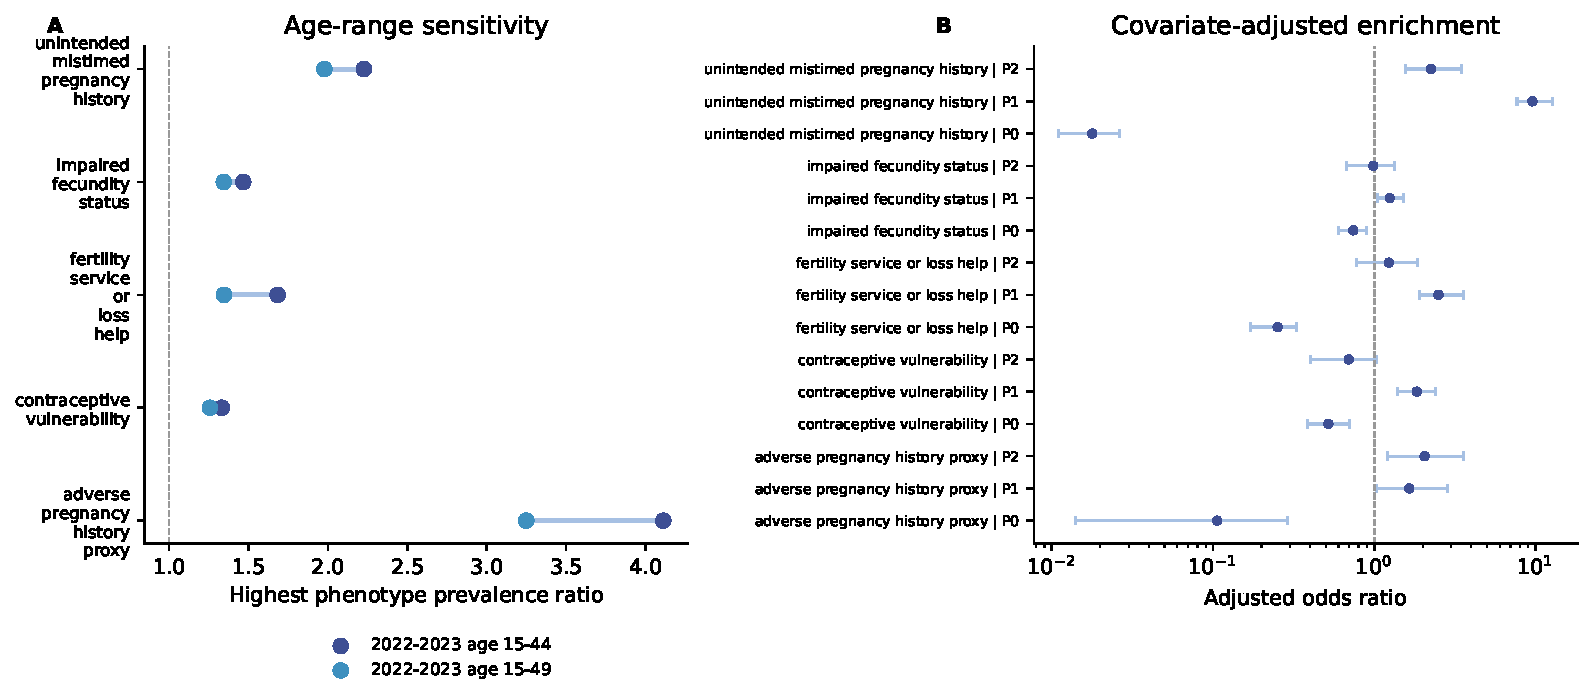
\includegraphics[width=\textwidth]{figures/supplementary_robustness_age_adjusted.pdf}
\caption{Robustness analysis for age-range sensitivity and covariate-adjusted endpoint enrichment. (A) Highest-phenotype prevalence ratios in 2022--2023 ages 15--44 versus 15--49 years. (B) Survey-weighted adjusted odds ratios from one-vs-rest phenotype enrichment models.}
\label{fig:supp_age_adjusted}
\end{figure}

\begin{figure}[H]
\centering
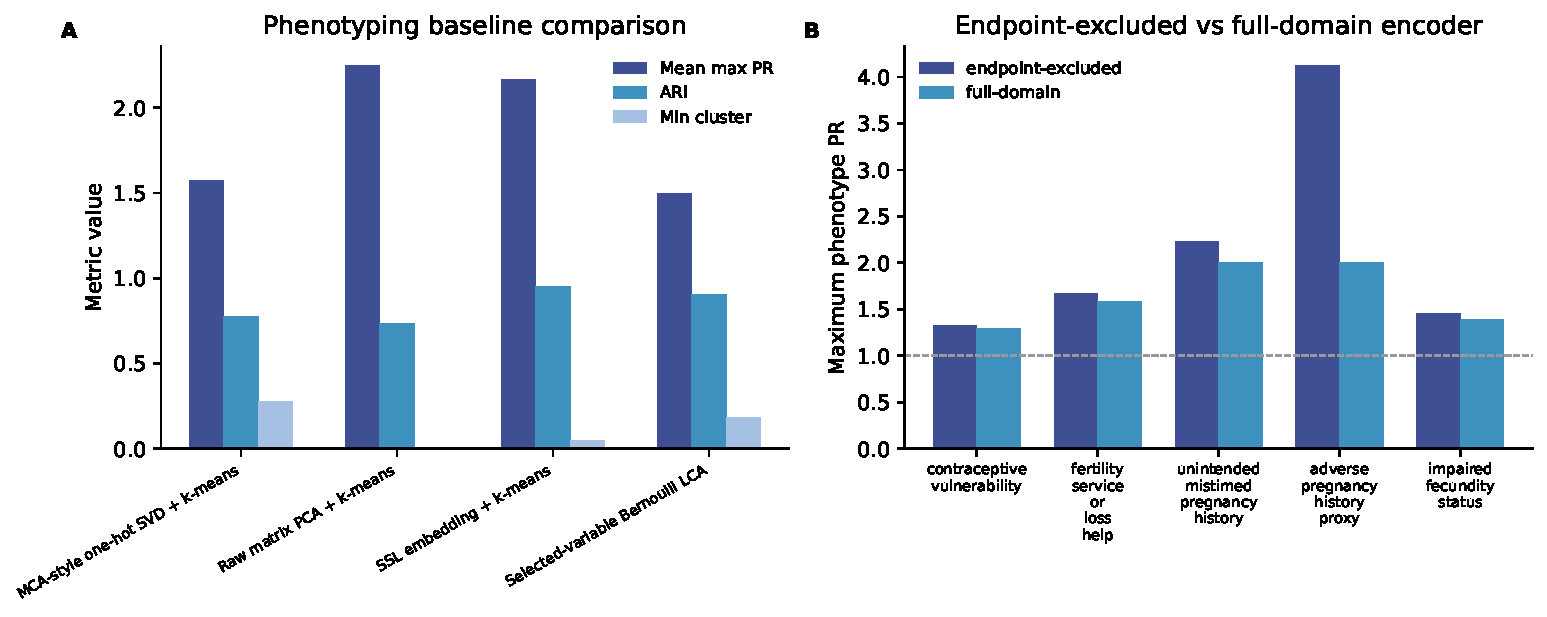
\includegraphics[width=\textwidth]{figures/supplementary_method_leakage_sensitivity.pdf}
\caption{Baseline-method and leakage-sensitivity analyses. (A) SSL phenotyping compared with raw PCA, MCA-style one-hot SVD, and selected-variable Bernoulli LCA baselines. (B) Maximum endpoint prevalence ratios for the primary endpoint-excluded encoder and a full-domain sensitivity encoder.}
\label{fig:supp_method_leakage}
\end{figure}

\begin{figure}[H]
\centering
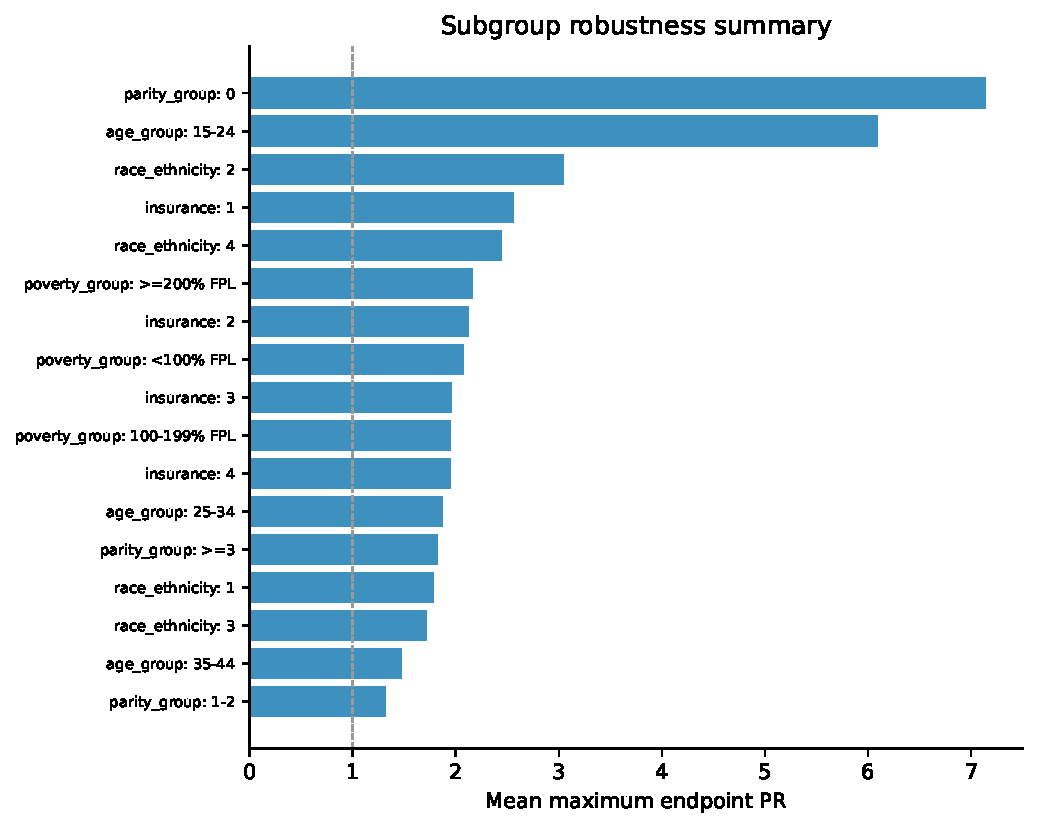
\includegraphics[width=0.8\textwidth]{figures/supplementary_subgroup_robustness.pdf}
\caption{Subgroup robustness summary across age, race/ethnicity, poverty, insurance, and parity strata. Values summarize mean maximum endpoint prevalence ratios by subgroup; subgroup categories use public-use recodes, and full decoded endpoint-by-phenotype estimates are included in source data and Supplementary Table S7.}
\label{fig:supp_subgroup}
\end{figure}

\begin{figure}[H]
\centering
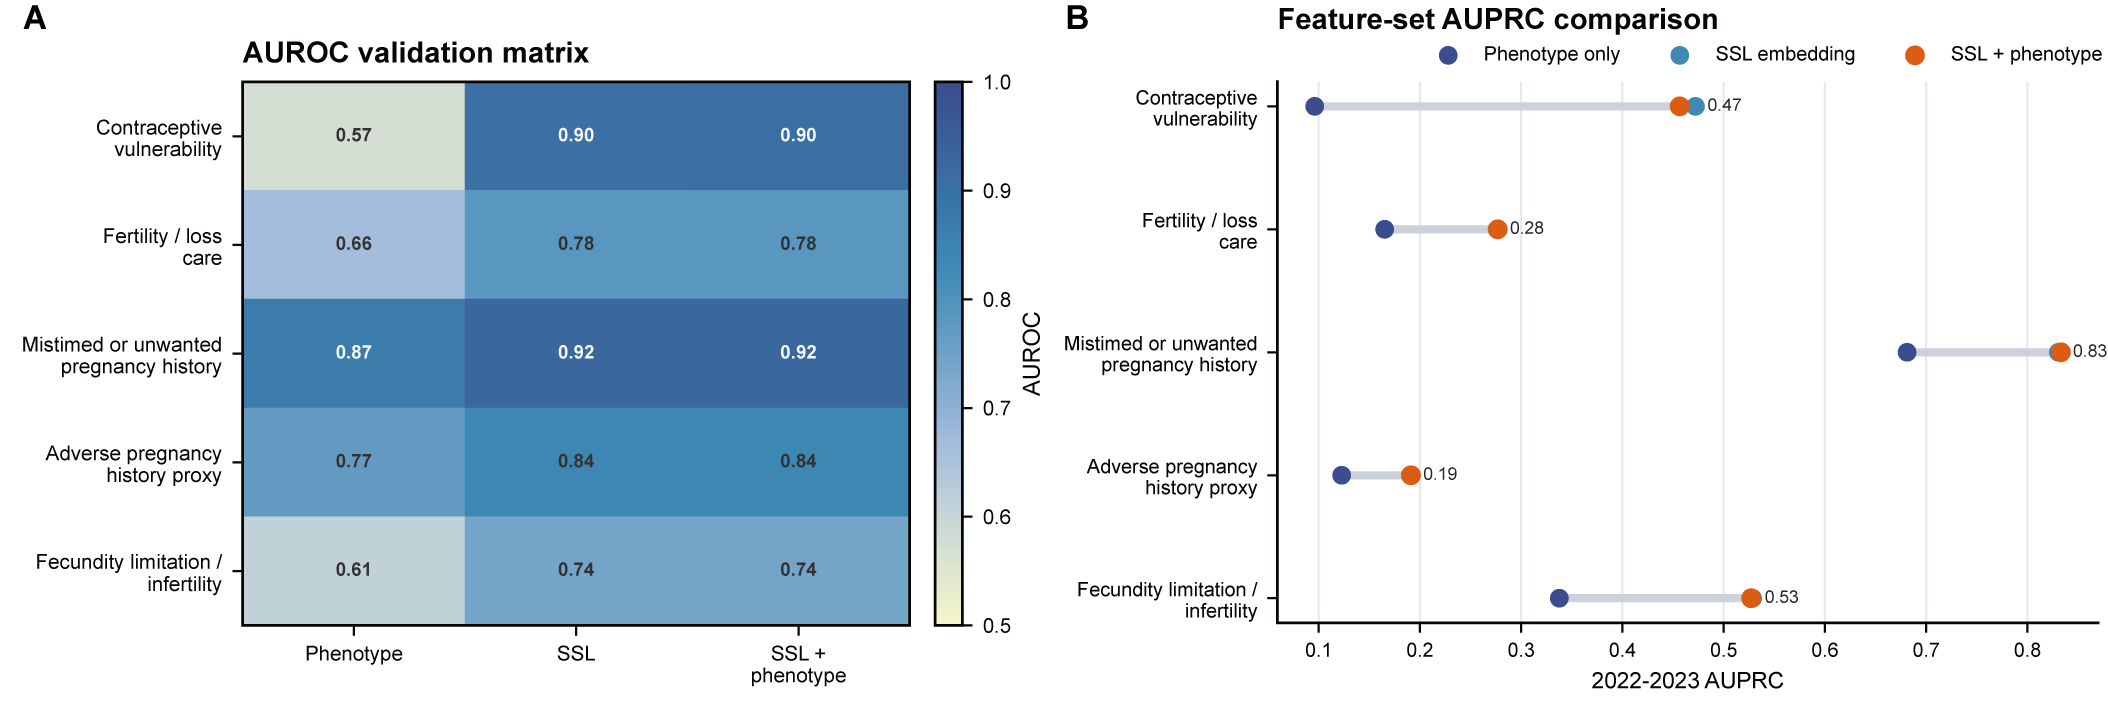
\includegraphics[width=\textwidth]{figures/FIG9.png}
\caption{Secondary supervised validation diagnostics. (A) AUROC validation matrix for phenotype-only, SSL-embedding, and SSL-plus-phenotype summaries across validation endpoints. AUROC is reported as a secondary discrimination summary and is not the primary claim. (B) Feature-set AUPRC comparison for phenotype-only, SSL-embedding, and SSL-plus-phenotype summaries. These diagnostics support representation and enrichment assessment rather than diagnostic prediction.}
\label{fig:model_diagnostics}
\end{figure}

\begin{figure}[H]
\centering
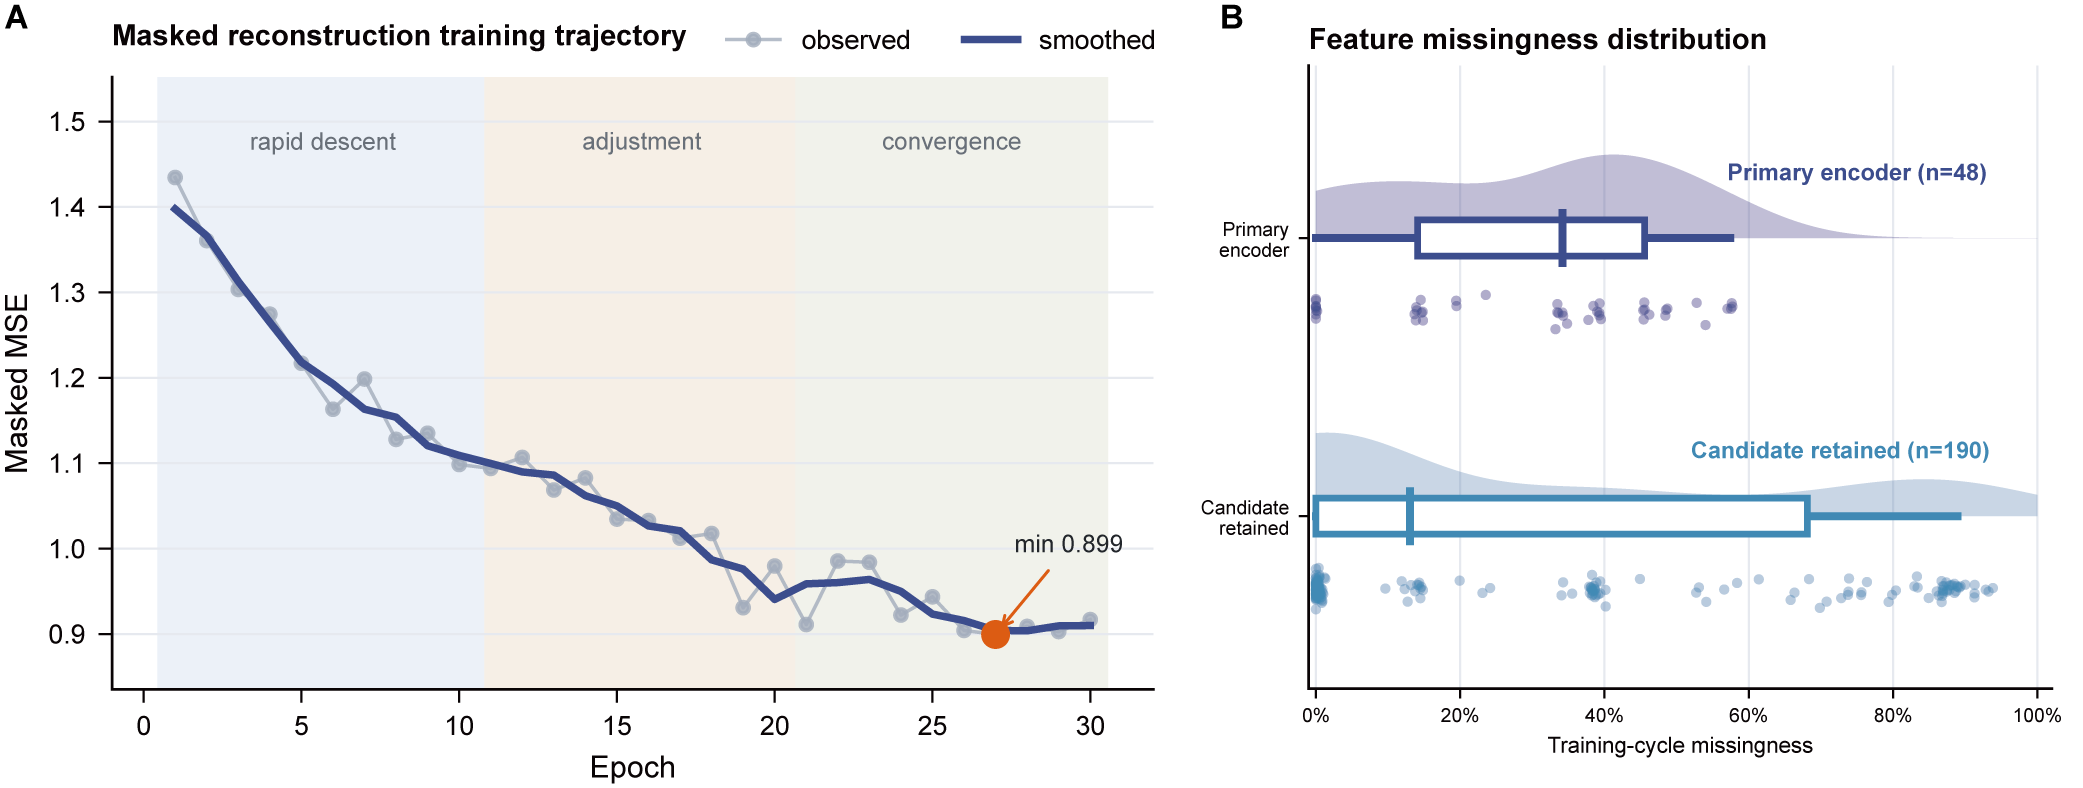
\includegraphics[width=\textwidth]{figures/FIG10.png}
\caption{SSL optimization and feature-missingness diagnostics. (A) Masked reconstruction loss across SSL training epochs, with rapid-descent, adjustment, and convergence phases, smoothed trend, and minimum-loss epoch annotation. (B) Distribution of training-cycle missingness among primary encoder features and retained candidate SSL features.}
\label{fig:ssl_diagnostics}
\end{figure}

\end{document}
